%%%%%%%%%%%%%%%%%%%%%%%%%%%%%%%%%%%%%%%%%%%%%%%%%%%%%%%%%%%%%%%%%%%%%%%%%%%%%%%%%%%%%%%%%%%%%%%%
%
% CS484 Written Question Template
%
% Acknowledgements:
% The original code is written by Prof. James Tompkin (james_tompkin@brown.edu).
% The second version is revised by Prof. Min H. Kim (minhkim@kaist.ac.kr).
%
% This is a LaTeX document. LaTeX is a markup language for producing 
% documents. Your task is to fill out this document, then to compile 
% it into a PDF document. 
%
% 
% TO COMPILE:
% > pdflatex thisfile.tex
%
% If you do not have LaTeX and need a LaTeX distribution:
% - Personal laptops (all common OS): www.latex-project.org/get/
% - We recommend latex compiler miktex (https://miktex.org/) for windows,
%   macTex (http://www.tug.org/mactex/) for macOS users.
%   And TeXstudio(http://www.texstudio.org/) for latex editor.
%   You should install both compiler and editor for editing latex.
%   The another option is Overleaf (https://www.overleaf.com/) which is 
%   an online latex editor.
%
% If you need help with LaTeX, please come to office hours. 
% Or, there is plenty of help online:
% https://en.wikibooks.org/wiki/LaTeX
%
% Good luck!
% Min and the CS484 staff
%
%%%%%%%%%%%%%%%%%%%%%%%%%%%%%%%%%%%%%%%%%%%%%%%%%%%%%%%%%%%%%%%%%%%%%%%%%%%%%%%%%%%%%%%%%%%%%%%%
%
% How to include two graphics on the same line:
% 
% \includegraphics[\width=0.49\linewidth]{yourgraphic1.png}
% \includegraphics[\width=0.49\linewidth]{yourgraphic2.png}
%
% How to include equations:
%
% \begin{equation}
% y = mx+c
% \end{equation}
% 
%%%%%%%%%%%%%%%%%%%%%%%%%%%%%%%%%%%%%%%%%%%%%%%%%%%%%%%%%%%%%%%%%%%%%%%%%%%%%%%%%%%%%%%%%%%%%%%%

\documentclass[11pt]{article}

\usepackage[english]{babel}
\usepackage[utf8]{inputenc}
\usepackage[colorlinks = true,
            linkcolor = blue,
            urlcolor  = blue]{hyperref}
\usepackage[a4paper,margin=1.5in]{geometry}
\usepackage{stackengine,graphicx}
\usepackage{fancyhdr}
\setlength{\headheight}{15pt}
\usepackage{microtype}
\usepackage{times}
\usepackage{booktabs}
\usepackage{float}

% From https://ctan.org/pkg/matlab-prettifier
\usepackage[numbered,framed]{matlab-prettifier}

\frenchspacing
\setlength{\parindent}{0cm} % Default is 15pt.
\setlength{\parskip}{0.3cm plus1mm minus1mm}

\pagestyle{fancy}
\fancyhf{}
\lhead{Homework Writeup}
\rhead{CS484}
\rfoot{\thepage}

\date{}

\title{\vspace{-1cm}Homework 5 Writeup}


\begin{document}
\maketitle
\vspace{-3cm}
\thispagestyle{fancy}

\section*{Instructions}
\begin{itemize}
  \item Describe any interesting decisions you made to write your algorithm.
  \item Show and discuss the results of your algorithm.
  \item Feel free to include code snippets, images, and equations.
  \item Use as many pages as you need, but err on the short side If you feel you only need to write a short amount to meet the brief, th
  
  \item \textbf{Please make this document anonymous.}
\end{itemize}

\section*{Algorithm Implementation}
Algorithms of this project is implemented in five parts. 

\subsection{Tiny Image Features}
Tiny image creation is simply resizing and normalization of images of the provided paths. Full code is shown below. In line 4, the list of image features is initialized with length same as the number of image paths. Then all the paths are iterated. In line 6, image is read. In line 7, image is reshaped in to a \emph{1*(16*16)} matrix. It is normalized in lines 8 and 9. Then it is added to the array in line 10.
\begin{lstlisting}[style=Matlab-editor]
function image_feats = get_tiny_images(image_paths)

imsize = 16;
image_feats = zeros(size(image_paths,1), imsize*imsize);
for i = 1:size(image_paths,1)
	img = imread(image_paths{i});
	img = double(reshape(imresize(img, [imsize, imsize]), 1, []));
	img = img - mean(img);
	img = img./norm(img);
	image_feats(i,:) = img;
end

end
\end{lstlisting}
\subsection{Nearest Neighbor Classification}
The k-NN classification works by letting k nearest neighbors "vote". Test images are classified with respect to train images by calculating pairwise distances. This is done in line 4. Then the distances are sorted in ascending order to find the closest points in line 5. The for loop is iterated through all test images. In liness 11 and 12, labels of k closest images are found. In lines 13 to 15, the label with most votes is found using a histogram added to the matrix.
\begin{lstlisting}[style=Matlab-editor]
function predicted_categories = nearest_neighbor_classify(train_image_feats, train_labels, test_image_feats, k)

N = size(test_image_feats,1);
pd = pdist2(train_image_feats, test_image_feats);
[~, sortindex] = sort(pd,1,'ascend');

labels = categorical(unique(train_labels));
predicted_categories = cell(N,1);

for i=1:N
	top_sort = sortindex(1:k,i);
	top_labels = categorical(train_labels(top_sort));
	[label_votes,elected] = histcounts(top_labels, labels);
	[~,mx_idx] = max(label_votes, [], 2);
	predicted_categories(i,:) = elected(mx_idx);
end

end
\end{lstlisting}

\subsection{Building Vocabulary}
Image vocabulary is built from points of certain cell size in all the images. The grid of points are created in lines 6 and 7. For each image, HOG features are found and added to the features in lines 18 and 19. Such matrix of features is clustered in line 22 to create vocabulary. Each cluster are the words.
\begin{lstlisting}[style=Matlab-editor]
function vocab = build_vocabulary(image_paths, vocab_size, cs, itv)

N = size(image_paths, 1);

cell_size = [cs cs];
[pv,ph] = meshgrid(cell_size(1)+1:itv:256, cell_size(2)+1:itv:256);
points = reshape(cat(3, pv,ph),size(pv,1)*size(pv,2),2);

feats = [];

for i = 1:N
	if (mod(i,100)==0)
		disp(i);
	end
	img = im2single(imread(image_paths{i}));
	img = imresize(img, [256 256]);
	
	[feature_vector,~] = extractHOGFeatures(img,points, 'CellSize',cell_size);
	feats = cat(1,feats,feature_vector);
end
size(feats)
[~,vocab] = kmeans(feats,vocab_size,'MaxIter',20000);
size(vocab)
end
\end{lstlisting}
\subsection{Bag of Words}
In this section, points are generated the same way as done in the previous section. Full code shown below. For each image, HOG feature is extracted in line 20. It is then searched using k-NN search from the vocabulary in line 22. The histogram of clusters is calculated and added to the image features array in line 23. 
\begin{lstlisting}[style=Matlab-editor]
function image_feats = get_bags_of_words(image_paths, cs, itv)

load('vocab.mat')
vocab_size = size(vocab, 1);
image_count = size(image_paths, 1);
image_feats = zeros(image_count, vocab_size);

forest = KDTreeSearcher(vocab);
cell_size = [cs cs];
[pv,ph] = meshgrid(cell_size(1)+1:itv:256, cell_size(2)+1:itv:256);
points = reshape(cat(3, pv,ph),size(pv,1)*size(pv,2),2);

for i=1:image_count
	if (mod(i,500)==0)
		disp(i);
	end
	img = im2single(imread(image_paths{i}));
	img = imresize(img, [256 256]);
	
	[features, ~] = extractHOGFeatures(img,points, 'CellSize', cell_size);
	
	[idx , ~] = knnsearch(forest , double(features), 'K', 1);
	image_feats(i,:) = histc(idx, 1:1:vocab_size)';
	end

end
\end{lstlisting}
\subsection{SVM Classification}
In this section, a multi-class SVM classification is implemented using multiple binary SVM classifiers. The unique categories are found in line 2. Then for each category, label was found line lines 8 and 9. Where the labels match are assigned 1 and -1 for the rest. The model is fit using the labels in line 11. The images are classified with the model in line 12. The respective scores are stored in a score matrix. After the binary classifications are done, the maximum scores are found and the corresponding category is returned in lines 16 and 18.

\begin{lstlisting}[style=Matlab-editor]
function predicted_categories = svm_classify(train_image_feats, train_labels, test_image_feats)
categories = unique(train_labels);
num_categories = length(categories);
scores = zeros(size(test_image_feats,1),num_categories);

for i=1:num_categories
	% two-class SVM for each category
	labels = double(strcmp(categories(i), train_labels));
	labels(labels==0) = -1;
	
	M = fitcsvm(train_image_feats, labels);
	[~,score] = predict(M,test_image_feats);
	scores(:,i) = score(:,2);
end

[~, max_idx] = max(scores,[],2);
size(max_idx)
predicted_categories = categories(max_idx');
end
\end{lstlisting}

\section*{Results}
Tiny image with nearest neighbor classifier achieved an accuracy of 0.214. Bag of words with nearest neighbor classifier had 0.439. Bag of words with SVM had 0.625. Figure~\ref{fig:conf} shows the confusion matrices of each cases.\\
\begin{figure}[H]
	\centering
	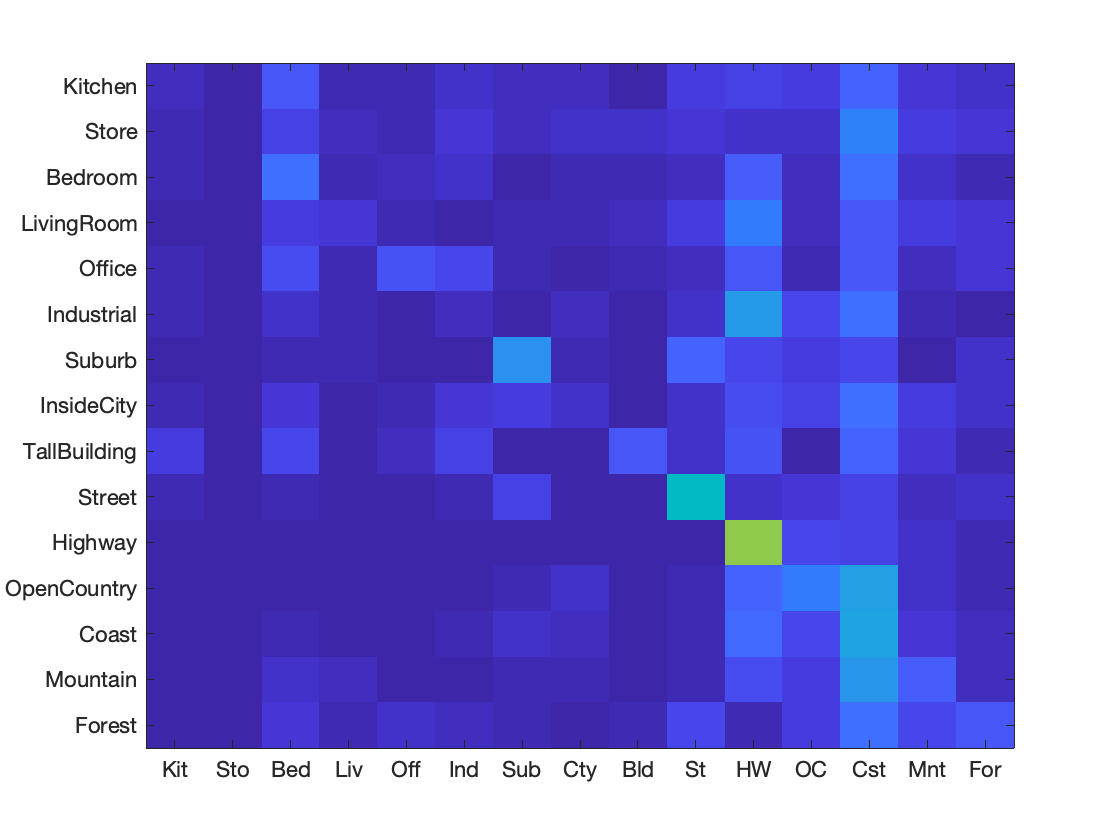
\includegraphics[width=0.3\textwidth]{../code/ti_nn.png}
	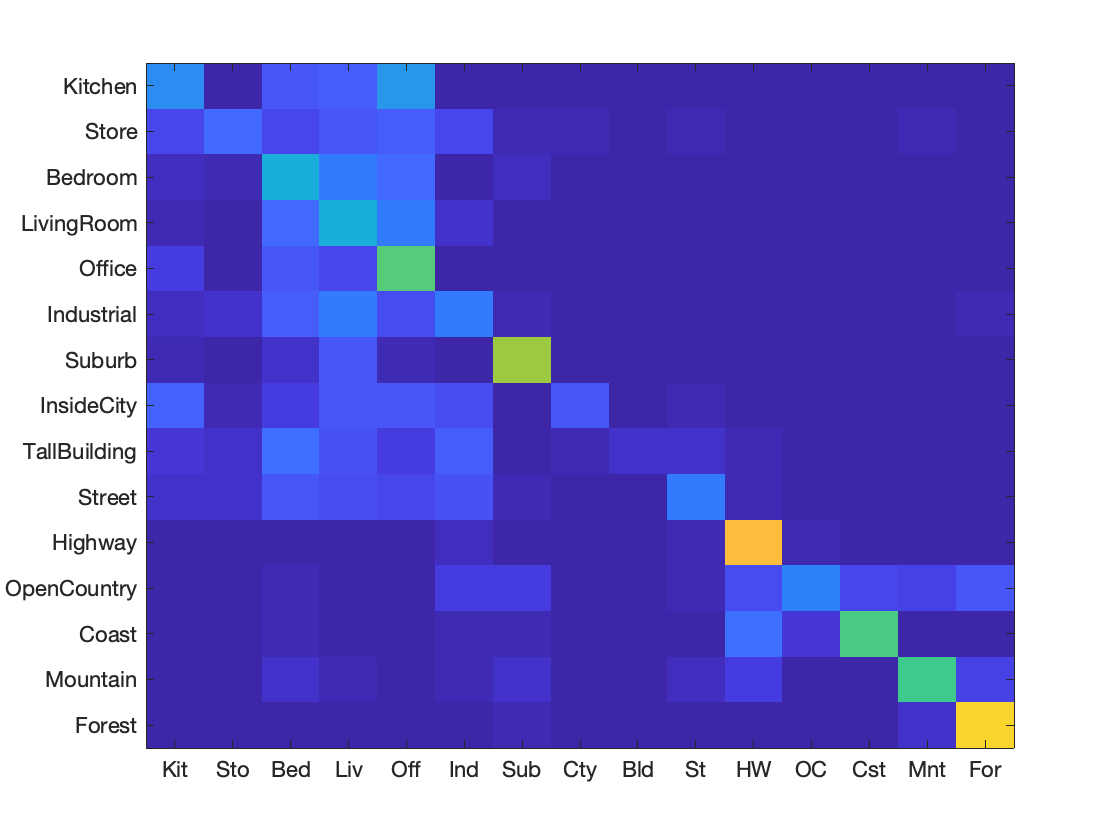
\includegraphics[width=0.3\textwidth]{../code/bw_nn.png}
	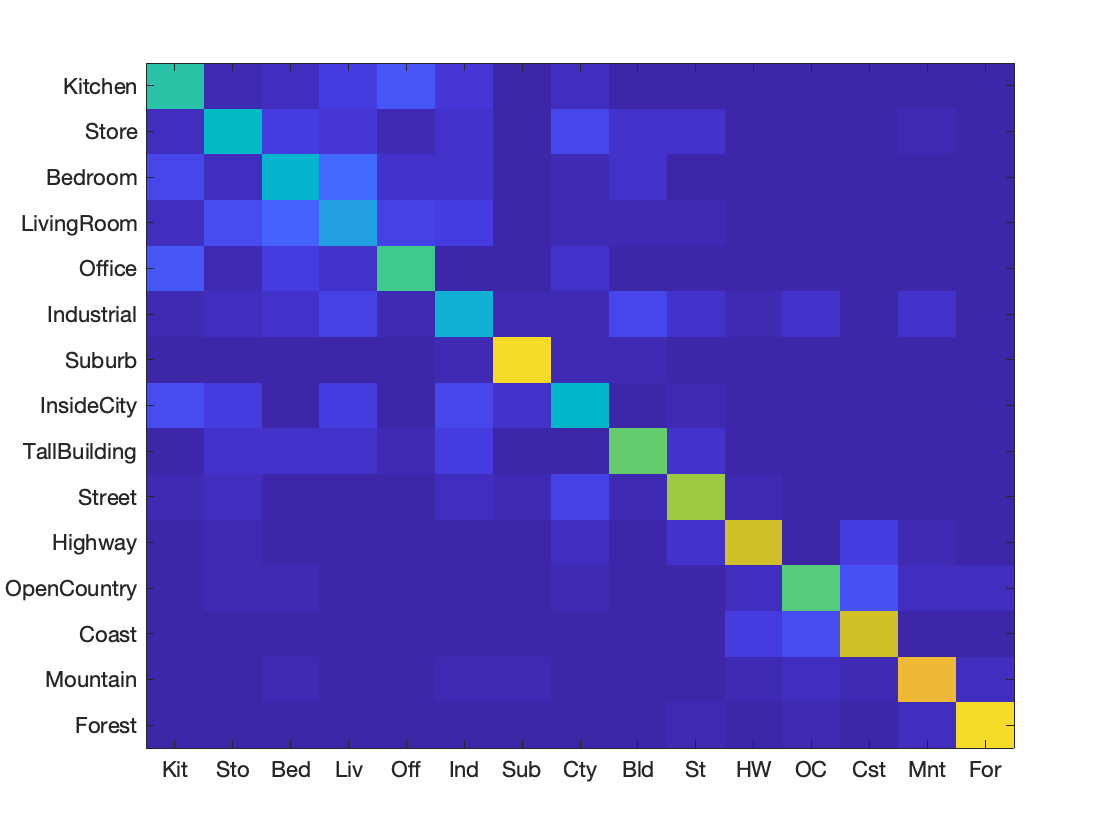
\includegraphics[width=0.3\textwidth]{../code/bw_svm.png}
	\caption{\emph{Left:} Tiny image with nearest neighbor classifier \emph{Middle:} Bag of words with nearest neighbor classifier. \emph{Right:} Bag of words with SVM classifier}
	\label{fig:conf}
\end{figure}
To maximize the accuracy, different parameters were adjusted. In the bag of words method, the cell size and interval of points to extract features from were adjusted. Different values are tested for accuracy and the result shows in Figure~\ref{fig:size_adj}. The optimal value of cell size of 20 and interval of 16 was found. \\

\begin{figure}[H]
	\centering
	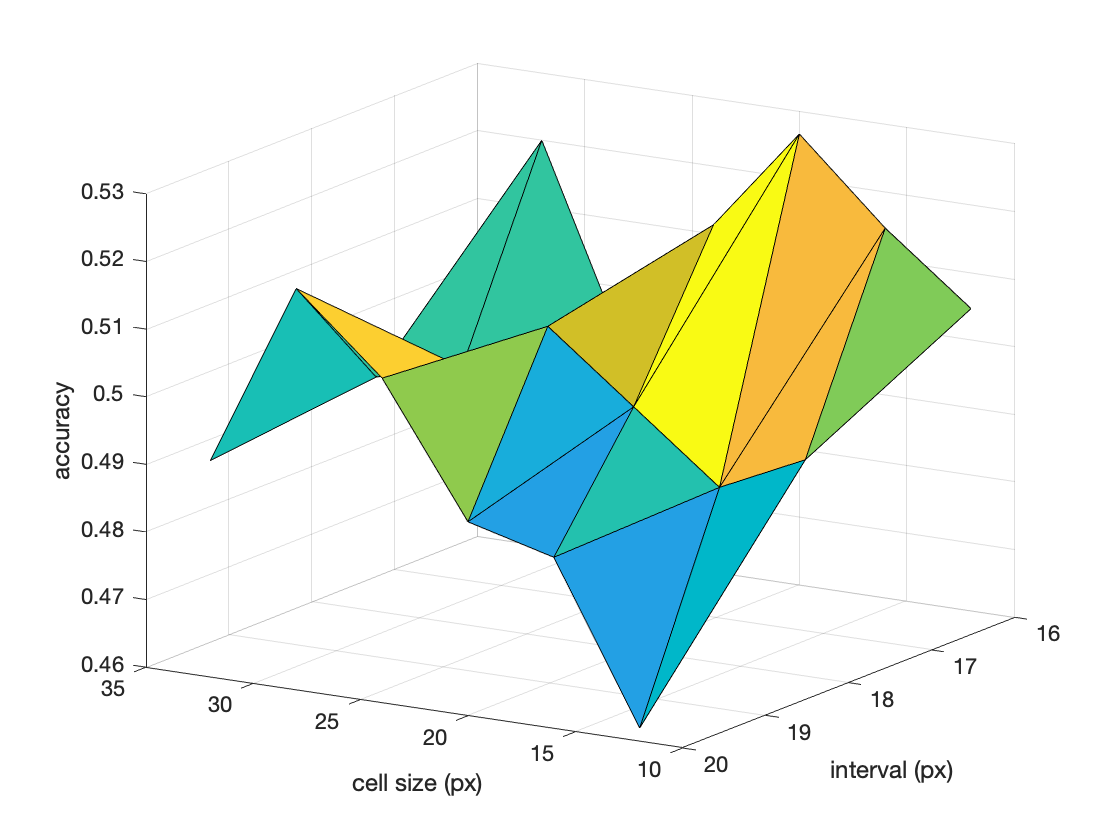
\includegraphics[width=0.45\textwidth]{../code/size_vs_acc.png}
	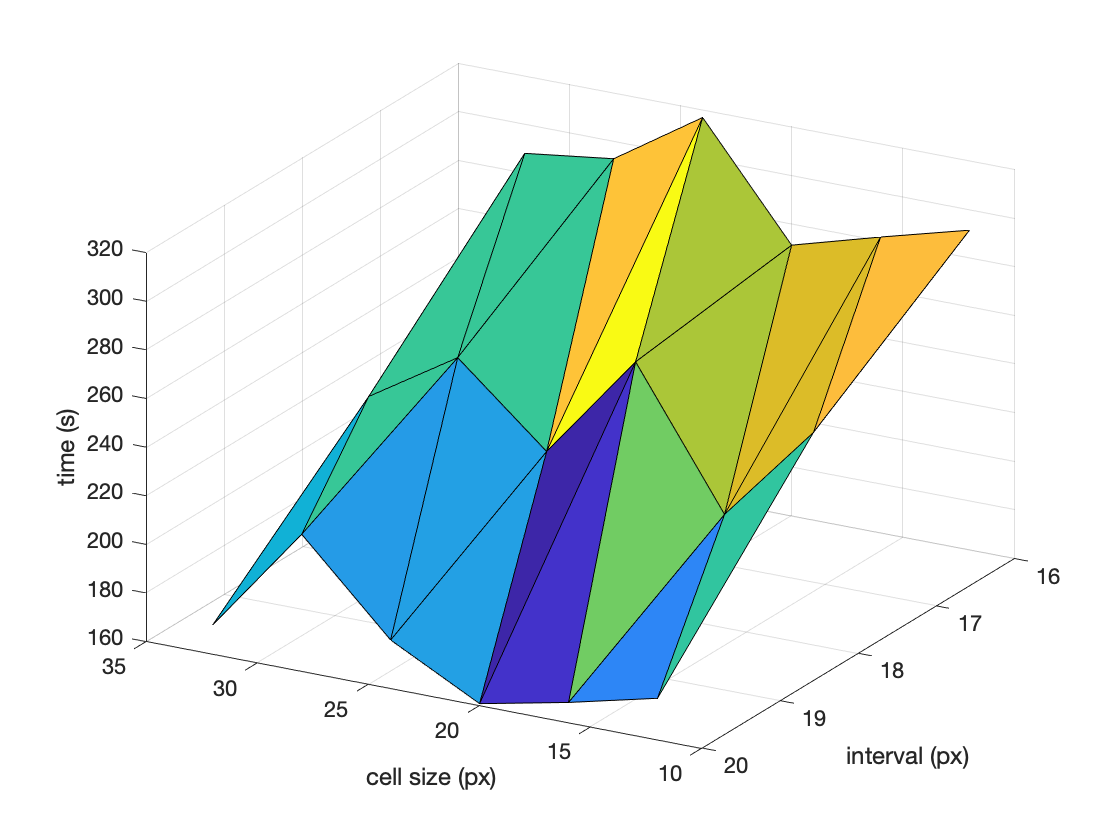
\includegraphics[width=0.45\textwidth]{../code/size_vs_time.png}
	\caption{\emph{Left:} Size vs Accuracy \emph{Right:} Size vs Time}
	\label{fig:size_adj}
\end{figure}

The vocabulary size is analyzed in Figure~\ref{fig:vocab}. The optimal vocabulary size was 1200. \\


\begin{figure}[H]
	\centering
	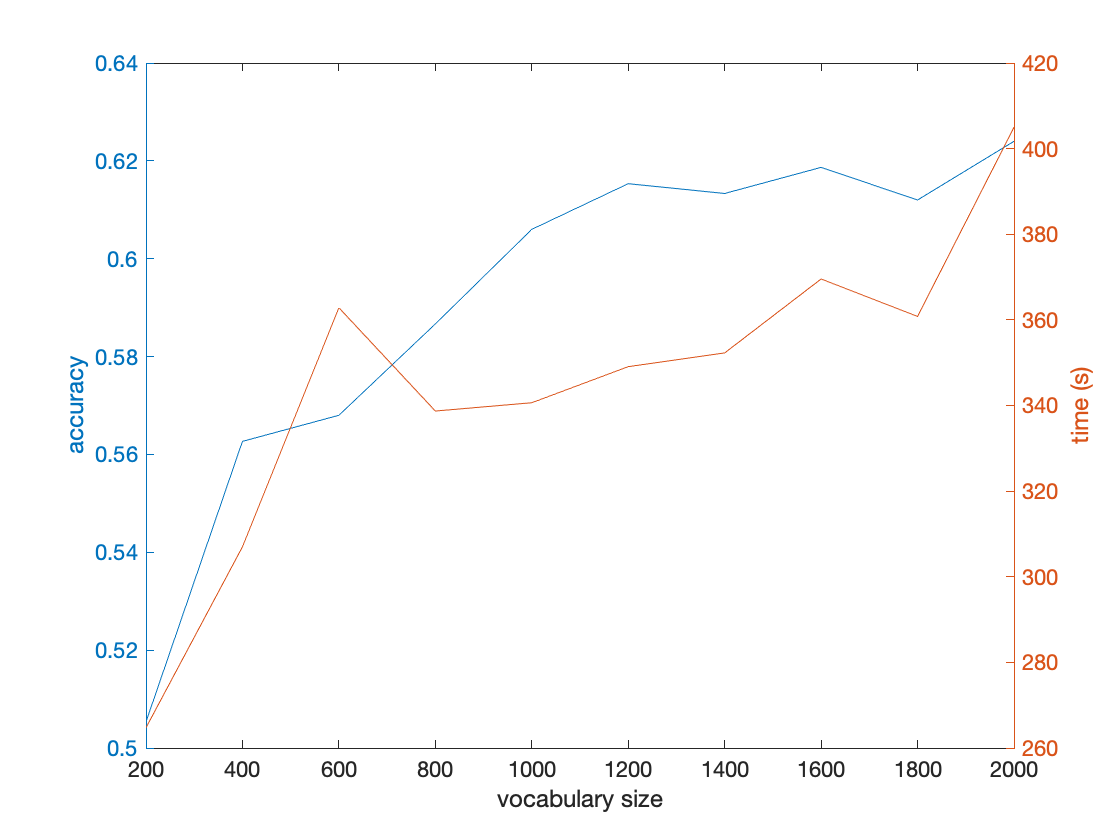
\includegraphics[width=0.6\textwidth]{../code/vocab_vs_acc.png}
	\caption{\emph{Left:} Size vs Accuracy and Time}
	\label{fig:vocab}
\end{figure}
The \emph{k} number is analyzed in Figure~\ref{fig:k_num}. The optimal \emph{k} number was 6.
\begin{figure}[H]
	\centering
	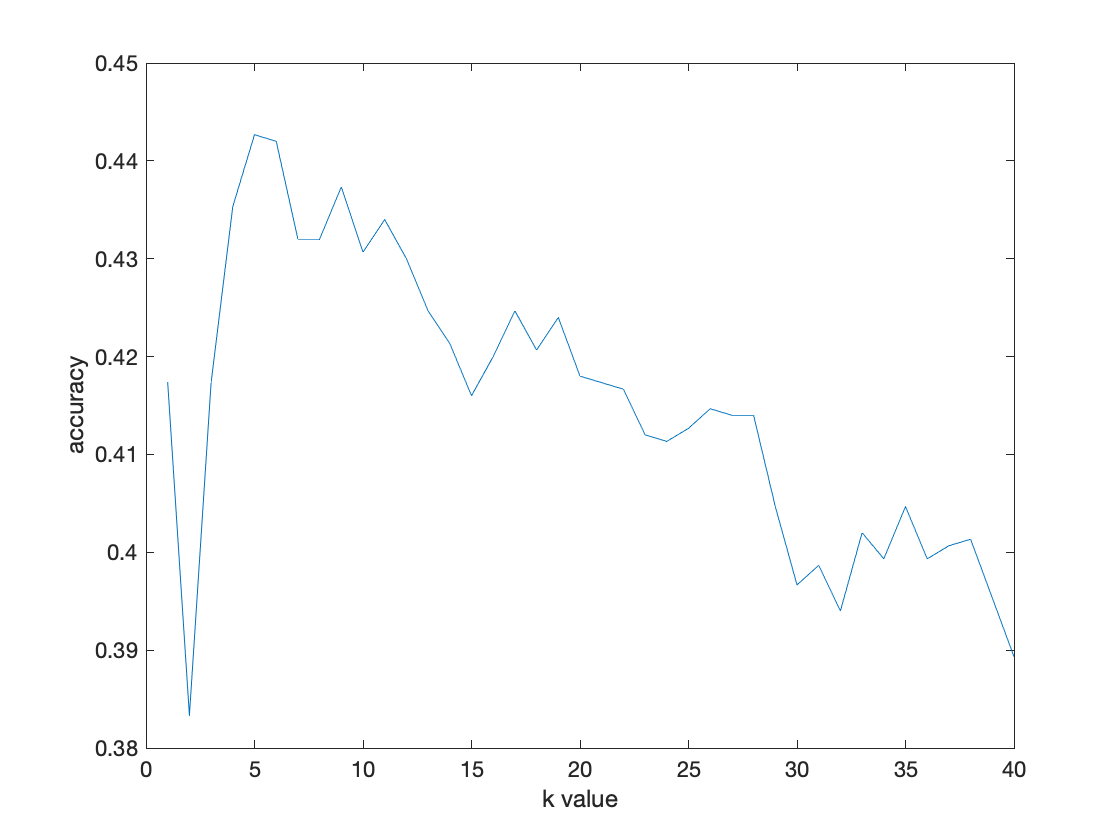
\includegraphics[width=0.6\textwidth]{../code/k_vs_acc.png}
	\caption{\emph{Left:} k value vs Accuracy}
	\label{fig:k_num}
\end{figure}

\end{document}
